\documentclass[12pt]{article}
\usepackage{amsmath}
\usepackage{amsfonts}
\usepackage{graphicx}
\DeclareGraphicsExtensions{.pdf,.png,.jpg}
\usepackage{algpseudocode}

\newtheorem{theorem}{Theorem}[section]
\newtheorem{lemma}[theorem]{Lemma}
\newtheorem{definition}[theorem]{Definition}


\title{Media Axis Sampling}
\date{}
\begin{document}
  \maketitle
  
  This is some media axis sampling outputs of algorithm mentioned in $\cite{steven}$. As mentioned last Tuesday, by changing the terminal condition a bit. We can sample spheres with any size.\\
  
  All the figures shown below are 800x800 sized. There are three rectangle obstacles in the middle of the 2d space. The space itself is white. All light gray areas are covered by no border discs. Black points are samples, as well as centers of discs.\\
  
  Figure \ref{fig:MA} shows the result of sampling on the media axis of the space. The result seems right. And as can be seen, almost the whole space is covered by discs centered at these media axis samples. 4 corners of the space are not well covered, we will talk about it later.\\ 
  
  We can also sample points in the space with any clearance. Figure \ref{fig:ISO} shows the result of sampling points 30(pixels) distance away from obstacles or the boundary of the space.\\
  
   All of the two figures contain 1000 samples( black points ). But they are not uniformly distributed on neither the media axis nor on the iso-cost contours. As can be seen in the pictures, samples near corner is much less than near obstacles. The reason is, the algorithm uniformly get random points in the space, and "push" them, along some direction, to the media axis. Therefore the probability of a narrow passage getting sampled depends on the volume of the passage, as well as the volume of its surrounding obstacles. Jory Denny $\cite{jory}$ mentioned a way to sample on media axis such that samples are uniformly distributed. By uniformly sampling, we can cover the corner of the space better. \\
  
  \begin{figure}[p]
  \centering
  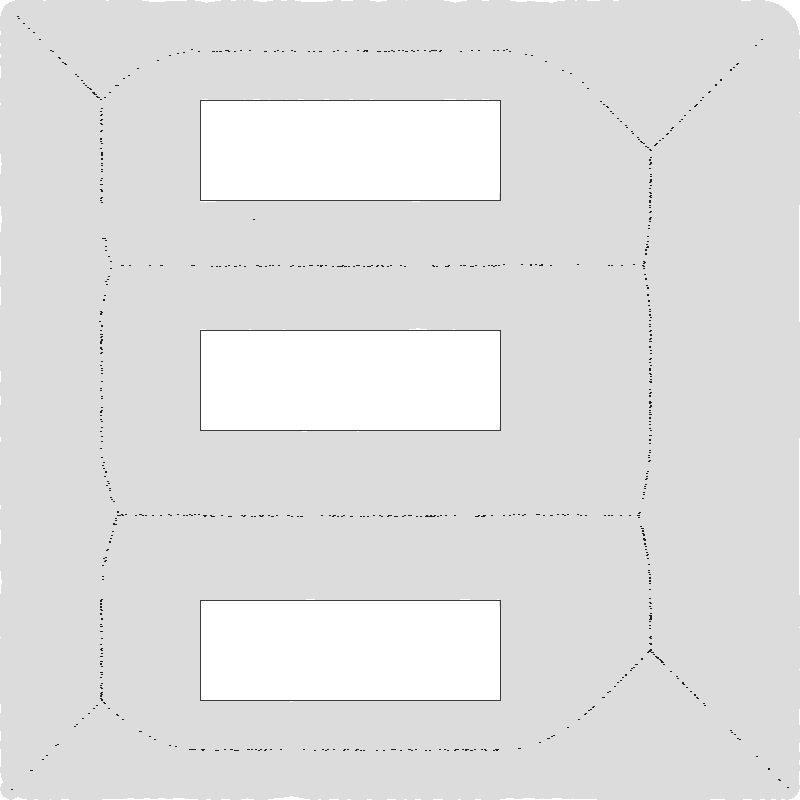
\includegraphics[scale=0.5]{MediaAxis_Cover.PNG}  
  \caption{Sampling on Media Axis}   
  \label{fig:MA} 
  \end{figure}
  
  \begin{figure}[p]
  \centering
  
\includegraphics[scale=0.5]{MediaAxis_cost_30.PNG}  
  \caption{Sampling on Media Axis}   
  \label{fig:ISO} 
  \end{figure}
        
  
  \begin{thebibliography}{1}

  \bibitem{steven} Steven A. Wilmarth, Nancy M. Amato, Peter F. Stiller. "MAPRM: A Probabilistic Roadmap Planner with Sampling on the Medial Axis of the Free Space", In Proc. IEEE Int. Conf. Robot. Autom. (ICRA), pp. 1024-1031, Detroit, MI, May 1999. Also, Technical Report, TR98-0022, Department of Computer Science and Engineering, Texas A \& M University, Nov 1998.

  \bibitem{jory} Jory Denny, Evan Greco, Shawna L. Thomas, Nancy M. Amato, "MARRT: Medial Axis Biased Rapidly-Exploring Random Trees",  In Proc. IEEE Int. Conf. Robot. Autom. (ICRA), Hong Kong, China, Jun 2014.

  \end{thebibliography}
  
\end{document}
  